\subsection{\label{subsec:A1}Röntgenstrahlabsorption}
\subsubsection{Kalibrierung}
Um die Messergebnisse, deren Gewinnung in Abschnitt 
\ref{subsec:vers1} beschrieben ist, nutzbar zu machen, muss zunächst 
der gemessene Beugungswinkel $\Theta$ mit der gebeugten Wellenlänge $\lambda$ 
in Verbindung gebracht werden. Hierzu verwenden wir die Braggsche 
Gleichung \eqref{eq:bragg} und die Berechnung des Netzebenenabstands, für 
welchen im kubischen System folgendes gilt
\begin{equation}
    d_{hkl} = \frac{a}{\sqrt{h^{2} + k^{2} + l^{2}}}.
\end{equation}
Da der Kristall so präpariert wurde, dass der Röntgenstrahl an der (220)-Ebene gebeugt wird,
folgt
\begin{align}
    d_{220} &\coloneqq d = \frac{a}{\sqrt{2^{2} + 2^{2} + 0^{2}}} \approx 1,931462\,\si{\angstrom} \\
    s_{d} &= \frac{s_{a}}{\sqrt{8}} \approx 0,000354\,\si{\angstrom} \\
    \Rightarrow \Aboxed{d &= (1,9315 \pm 0,0004)\,\si{\angstrom}}.
\end{align}
Der berechnete Fehler $s_{d}$ ist so gering, dass er für die weitere Berechnung keine Rolle spielt. \\
Aus Gl.~\eqref{eq:bragg} folgt 
\begin{align}
    \lambda &= \frac{2d}{n}\sin(\Theta)  \label{eq:welle} \\
    \Leftrightarrow \Theta &= \arcsin\left(\frac{n\lambda}{2d}\right), \label{eq:winkel}
\end{align}
womit wir die gemessenen Winkel in Wellenlängen und zurück rechnen können. \\
Weiterhin muss eine Winkelkalibrierung erfolgen, die den gemessenen Winkel mithilfe
theoretischer Referenzpunkte mit einem realen Winkel in Verbindung bringt. 
Bei einer idealen Justierung und einem perfekten Messaufbau könnte auf diesen Schritt 
verzichtet werden, hier aufgrund der benötigten Genauigkeit jedoch durchgeführt.
Die Referenzpunkte sind durch die charakteristische Röntgenstrahlung der Wolfram-Anode 
gegeben, wobei Tabelle 1 der Versuchsanleitung \cite{Anleitung} die erlaubten 
Übergänge auflistet. Rechnet man die theoretische Lage über Gl.~\eqref{eq:winkel} 
in Winkel um, an denen die Linien erwartet werden, so zeigt sich, dass die erste 
Beugungsordnung ($n=1$) der linken Spalte nicht im betrachteten Messbereich liegt. 
In Abb.~\ref{fig:kali} ist das gemessene Spektrum als Funktion des Messwinkels $\Theta_{\text{mess}}$
dargestellt und die beobachteten Linien, sowie deren Beugungsordnung eingezeichnet. \\
Drei der zehn theoretisch beobachtbaren Linien ($L\gamma_{3},\,L\eta,\,L\alpha_{2}$) 
können wir nicht identifizieren, was an einer 
geringen relativen Intensität und zu schlechtem Auflösungsvermögen des justierten Messaufbaus 
liegen kann \cite{xRay}. Für einige Linien ist bei großen Winkeln zusätzlich die zweite Beugungsordnung 
($n=2$ in Gl.~\eqref{eq:bragg}) zu erkennen. \\ 
Mithilfe der identifizierten Linien lässt sich nun der kalibrierte Beugungswinkel $\Theta_{\text{kali}}$ 
errechnen, indem die theoretische und die gemessene Winkellage gegeneinander aufgetragen wird und eine 
Gerade gefittet wird, welche die lineare Transformation zwischen kalibriertem und gemessenen Winkel beschreibt.
Es gilt
\begin{equation}
    \Theta_{\text{kali}} = m\cdot\Theta_{\text{mess}} + b,
\end{equation} 
wobei aufgrund der gegebenen Linearität der Messgeräte eine Steigung nahe eins erwartet wird. 
Der Achsenabschnitt $b$ gibt Information über einen globalen Shift der Winkelmessung, der für 
genaue Messungen notwendigerweise korrigiert werden muss. \\
Aus dem, mit Python durchgeführten, Fit erhalten wir folgende Werte inklusive ihrer errechneten 
Standardabweichungen $s$
\begin{alignat}{3}
    m &= 0.9984761 \hspace{1.5cm}&s_{m} = 0.0018515 \hspace{1.5cm} \Rightarrow&\Aboxed{m = (0.998\pm0.002)} \\
    b &= 0.1030292 \hspace{1.5cm}&s_{b} = 0.0529446 \hspace{1.5cm} \Rightarrow&\Aboxed{b = (0.10\pm0.05)^{\circ}}.
\end{alignat}   
Die dazugehörige Grafik ist in Abb.~\ref{fig:fitkali} dargestellt. \newpage
\begin{figure}[h!]
    \centering
    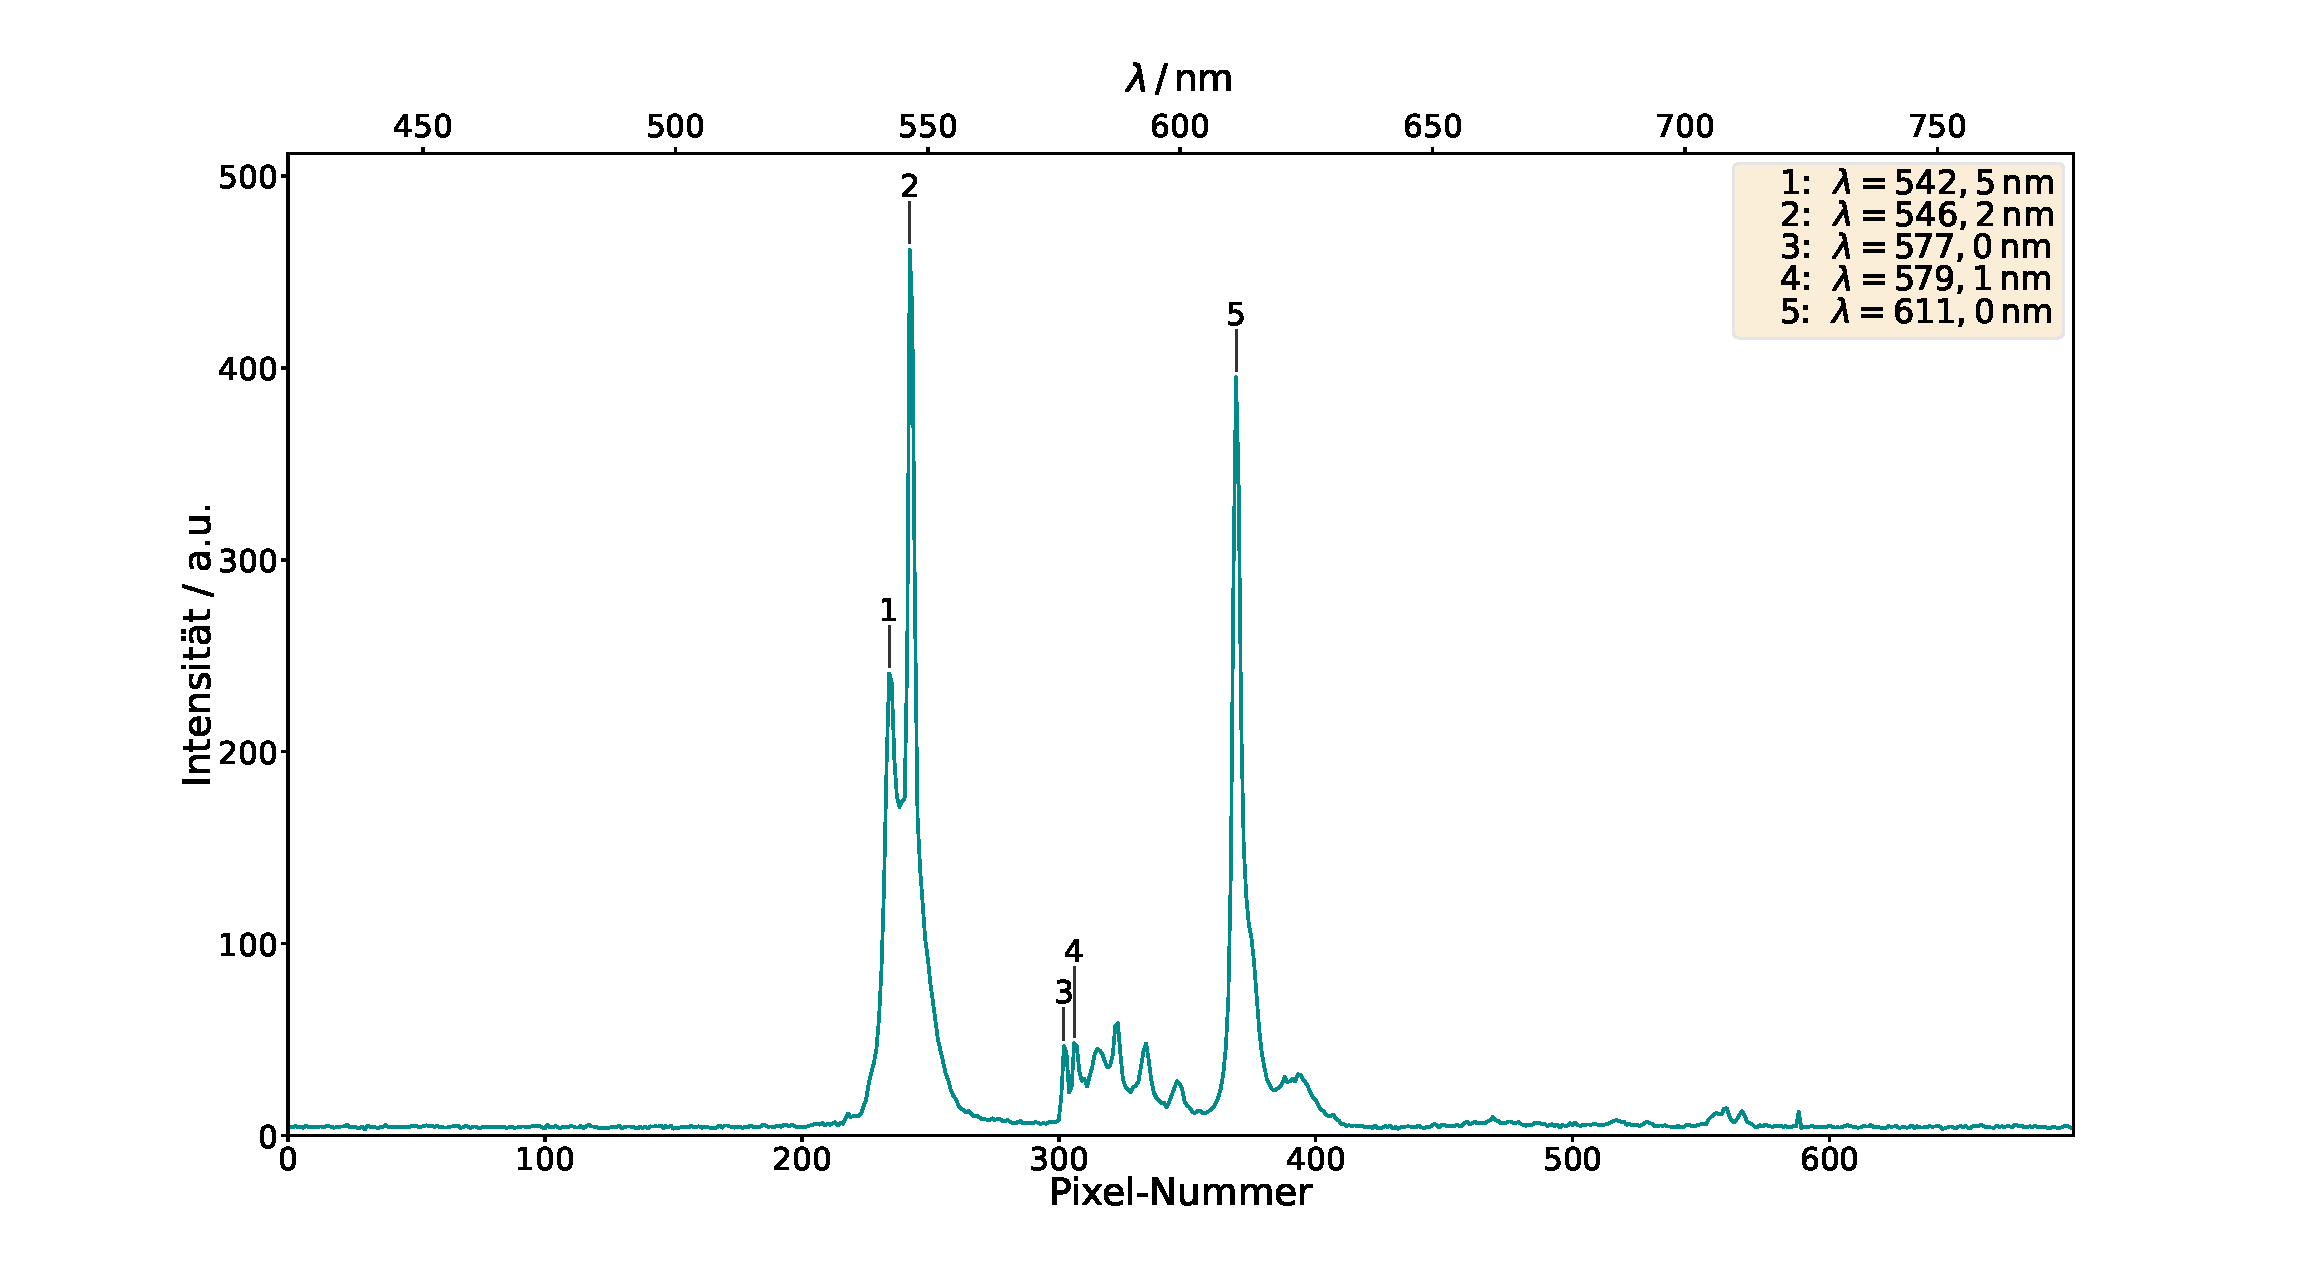
\includegraphics[clip, trim={3cm 1cm 3cm 2.5cm}, width=\textwidth]{Kalib.pdf}
    \caption{\label{fig:kali}Die gemessene Photonenanzahl als normierte Intensität gegen den 
    gemessenen Winkel $\Theta_{\text{mess}}$ aufgetragen. Zusätzlich sind die 
    beobachtbaren charakteristischen Linien eingezeichnet und identifiziert. 
    Der erste erkennbaren Peak (direkt neben 1) konnte nicht eindeutig identifiziert werden,
    weswegen dieser für weitere Berechnungen ignoriert wird.}
\end{figure}\FloatBarrier
\begin{figure}[h!]
    \centering
    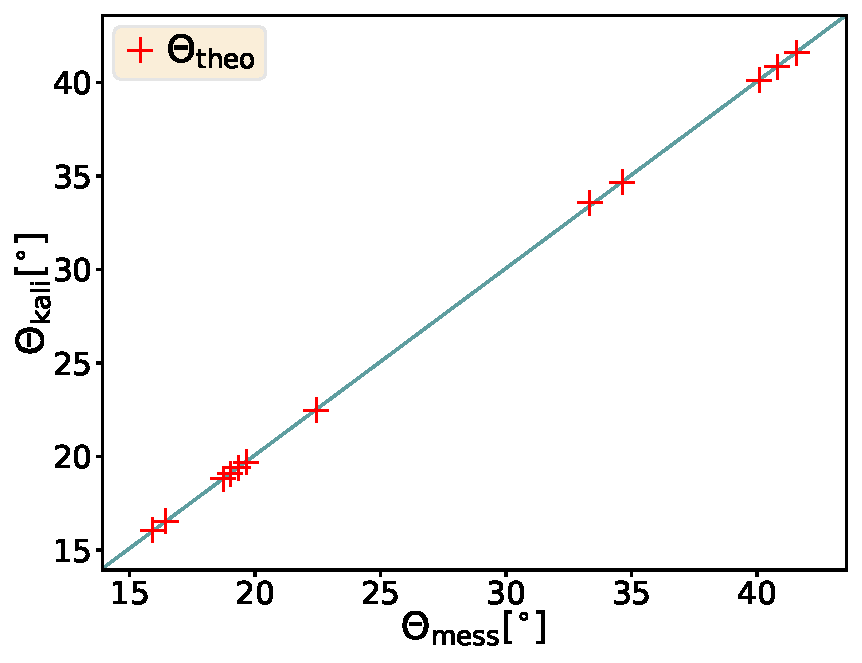
\includegraphics[width=0.6\textwidth]{fit.pdf}
    \caption{\label{fig:fitkali}Die theoretische Lage der identifizierten Linien gegen 
    die gemessene Lage aufgetragen. Zusätzlich ist eine Gerade zur Kalibration der gemessenen 
    Winkel durch die Werte gelegt. Aufgrund der Übersichtlichkeit wir nur der relevante 
    Bereich dargestellt, während der Achsenabschnitt im Haupttext dargestellt ist.}
\end{figure}\FloatBarrier
Aus dem errechneten Wert der Steigung kann man auf Linearität der Messgeräte schließen, da sie innerhalb 
des Fehlers die Identität bildet. Der Achsenabschnitt ist nicht vernachlässigbar, weist jedoch einen
hohen Fehler auf. \\
Die Korrektur des gemessenen Beugungswinkels wird trotz der erhaltenen Linearität 
mit beiden Werten durchgeführt, was unter 
Benutzung von Gl.~\eqref{eq:welle} zum gewünschten Spektrum führt. 
Zu beachten ist hierbei die Fehlerfortpflanzung des linearen Fits, was zu folgendem 
Fehler der Wellenlänge führt
\begin{align}
    s_{\lambda} &= \left\vert\frac{\partial \lambda}{\partial \Theta}\right\vert = \left\vert2d\cos(\Theta)s_{\Theta}\right\vert \\
    s_{\Theta} &= \sqrt{\left(\Theta_{\text{kali}}s_{m}\right)^{2} + s_{b}^{2}}.
\end{align}
Dieser Wert muss bei der folgenden Kantenbestimmung zusätzlich zum Ablesefehler berücksichtigt werden.
\subsubsection{Identifizierung des Metallplättchens}





